\documentclass[letterpaper,10pt]{article}

\usepackage{tabularx} % extra features for tabular environment
\usepackage{amsmath}  % improve math presentation
\usepackage{graphicx} % takes care of graphic including machinery
\usepackage[margin=1in,letterpaper]{geometry} % decreases margins
\usepackage{cite} % takes care of citations
\usepackage[final]{hyperref} % adds hyper links inside the generated pdf file
\usepackage{ctex}
\usepackage{titlesec}
%\usepackage{CJKutf8, CJK}
\usepackage{makecell}                 % 三线表-竖线
\usepackage{booktabs}                 % 三线表-短细横线
% \usepackage{natbib}
\usepackage{graphicx}				  % 表格单元格逆时针
\usepackage{multirow}				  % 合并单元格
\usepackage{array}
\usepackage{amssymb}				  % 勾
\usepackage{amsmath}
\usepackage{longtable}                % 导入 longtable 宏包,表格自动换行
\usepackage{caption}
\usepackage{subcaption}               % 设置子图
\usepackage{color}					  % 文本颜色包
\usepackage{xcolor}
\usepackage{bbm}					  % 输入指示函数
\usepackage{tablefootnote}			  % 表格注释
\usepackage{pythonhighlight}
\usepackage{fancyhdr}
\usepackage{lastpage}
\pagestyle{fancy}
\fancyhf{}
\fancyhead{}
\fancyfoot{}
\fancyhead[R]{\small Page \thepage\ of \pageref*{LastPage}}
\fancyhead[L]{\small Report}

\usepackage{listings}                 % 导入代码块
\usepackage{xcolor}
\lstset{
	numbers=left, 
	tabsize=1,
	columns=flexible, 
	numberstyle=  \small, 
	keywordstyle= \color{ blue!70},
	commentstyle= \color{red!50!green!50!blue!50}, 
	frame=shadowbox, % 阴影效果
	rulesepcolor= \color{ red!20!green!20!blue!20} ,
	escapeinside=``, % 英文分号中可写入中文
	xleftmargin=2em,
	xrightmargin=2em, 
	aboveskip=1em,
} 

\hypersetup{
	colorlinks=true,       % false: boxed links; true: colored links
	linkcolor=blue,        % color of internal links
	citecolor=blue,        % color of links to bibliography
	filecolor=magenta,     % color of file links
	urlcolor=blue         
}
%++++++++++++++++++++++++++++++++++++++++
\titleformat{\section}{\Large\bfseries\songti}{\thesection}{1em}{}
\titleformat{\subsection}{\large\bfseries\songti}{\thesubsection}{1em}{}
\titleformat{\subsubsection}{\normalsize\bfseries\songti}{\thesubsubsection}{1em}{}
\titleformat{\paragraph}{\small\bfseries\songti}{\paragraph}{1em}{}
\titleformat{\subparagraph}{\footnotesize\bfseries\songti}{\subparagraph}{1em}{}

\begin{document}
	
	
	\title{\songti \zihao{4}7月10日-7月16日工作汇报}
	\author{\textrm{Ku Jui}}
	\date{\textrm{July 2023}}
	\maketitle
	
	\renewcommand{\figurename}{Figure} % 可以重新定义abstract,因为ctex会覆盖thebibliography
	% 	\begin{abstract}
		%		In this experiment we studied a very important physical effect by measuring the
		%		dependence of a quantity $V$ of the quantity $X$ for two different sample
		%		temperatures.  Our experimental measurements confirmed the quadratic dependence
		%		$V = kX^2$ predicted by Someone's first law. The value of the mystery parameter
		%		$k = 15.4\pm 0.5$~s was extracted from the fit. This value is
		%		not consistent with the theoretically predicted $k_{theory}=17.34$~s. We attribute %this
		%		discrepancy to low efficiency of our $V$-detector.
		%	\end{abstract}
	\renewcommand{\contentsname}{Contents}
	\renewcommand{\tablename}{Table}
	\tableofcontents  % 自动生成目录
	
	\section{Pre-Knowledge}
		
	\subsection{Vision Transformer \cite{dosovitskiy2021image}}
	
	之前的算法大都是保持CNN整体结构不变,在CNN中增加attention模块或者使用attention模块替换CNN中的某些部分。ViT算法中,作者提出没有必要总是依赖于CNN,仅仅使用Transformer结构也能够在图像分类任务中表现很好。
	
	受到NLP领域中Transformer成功应用的启发,ViT算法中尝试将标准的Transformer结构直接应用于图像,并对整个图像分类流程进行最少的修改。具体来讲,ViT算法中,会将整幅图像拆分成小图像块,然后把这些小图像块的线性嵌入序列作为Transformer的输入送入网络,然后使用监督学习的方式进行图像分类的训练。ViT算法的整体结构如Fig.\ref{fig: Vision Transformer}所示。
	
	\begin{figure}[htbp]
		% read manual to see what [ht] means and for other possible options
		\centering 
		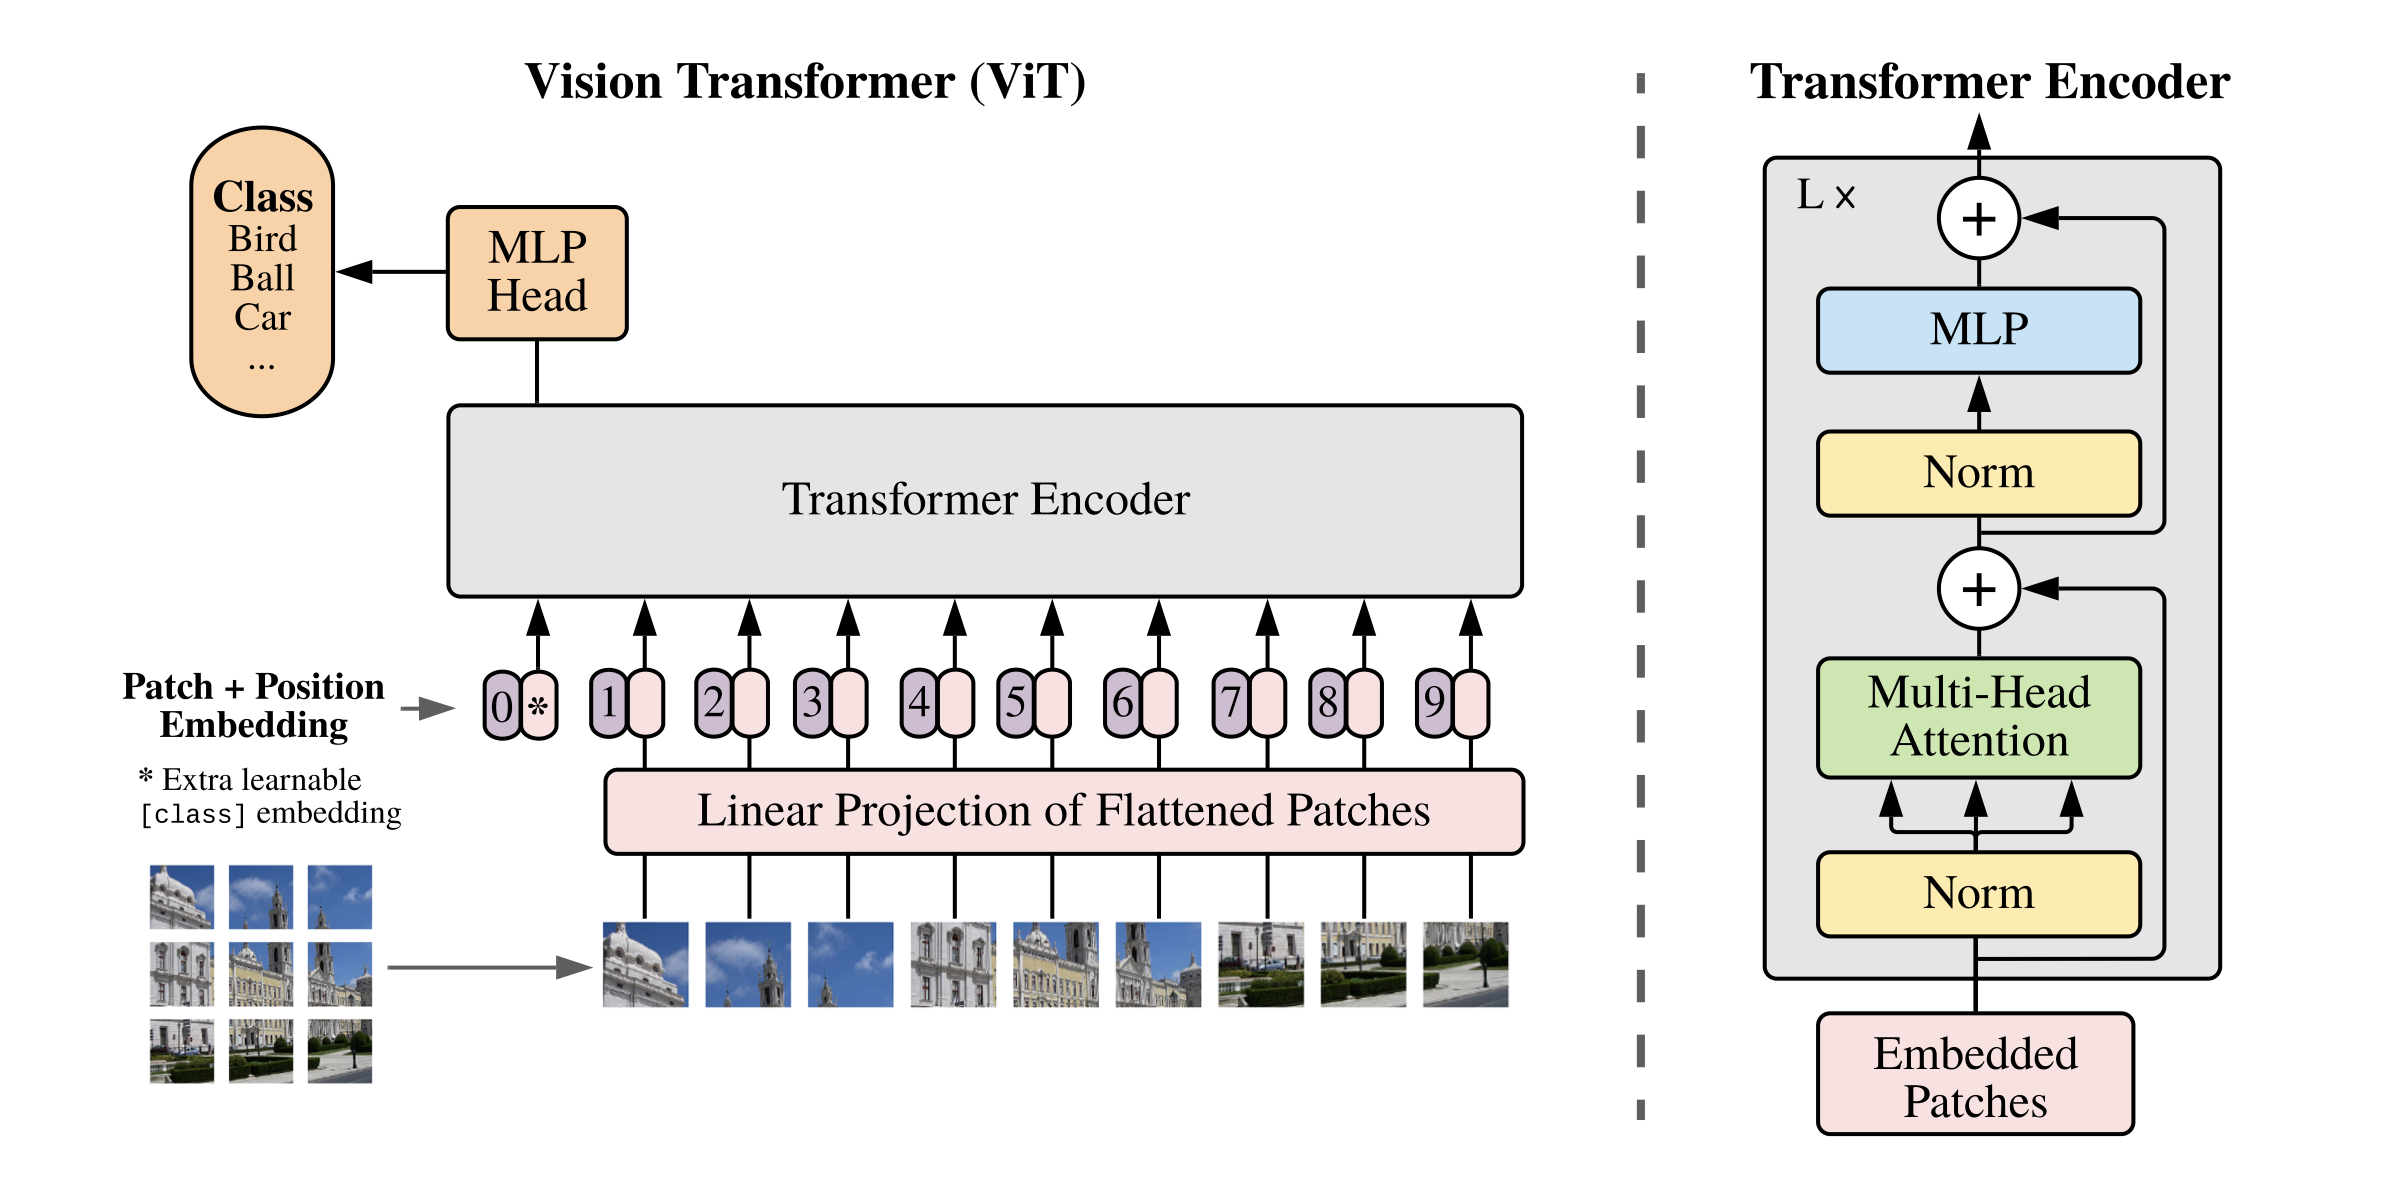
\includegraphics[width=0.8\columnwidth]{picture/Vision-Transformer-architecture}
		%\captionsetup{font=scriptsize}
		\caption{
			\label{fig: Vision Transformer} The Vision Transformer - model architecture.
		}
	\end{figure}
	
	
	该算法在中等规模(例如ImageNet)以及大规模(例如ImageNet-21K、JFT-300M)数据集上进行了实验验证,发现:
	
	\begin{itemize}
		\item {}
			Tranformer相较于CNN结构,缺少一定的平移不变性和局部感知性,因此在数据量不充分时,很难达到同等的效果。具体表现为使用中等规模的ImageNet训练的Tranformer会比ResNet在精度上低几个百分点。
		\item {}
			当有大量的训练样本时,结果则会发生改变。使用大规模数据集进行预训练后,再使用迁移学习的方式应用到其他数据集上,可以达到或超越SOTA水平。
	\end{itemize}
	
	Fig.\ref{fig: ViT precision}展示了使用大规模数据集预训练后的 ViT 算法,迁移到其他小规模数据集进行训练,与使用 CNN 结构的SOTA算法\footnote{BiT 与 Noisy Student 均为2020年提出的 SOTA 算法。
		\begin{itemize}
			\item {}
				BiT算法\cite{kolesnikov2020big}:使用大规模数据集 JFT-300M 对 \texttt{ResNet} 结构进行预训练,其中,作者发现模型越大,预训练效果越好,最终指标最高的为4倍宽、152层深的$\texttt{ResNet}152\times 4$。
			\item {}
				Noisy Student 算法\cite{xie2020self}:使用知识蒸馏的技术,基于 \texttt{EfficientNet} 结构,利用未标签数据,提高训练精度。
		\end{itemize}	
	}精度对比。
	
	
	\begin{figure}[htbp]
		% read manual to see what [ht] means and for other possible options
		\centering 
		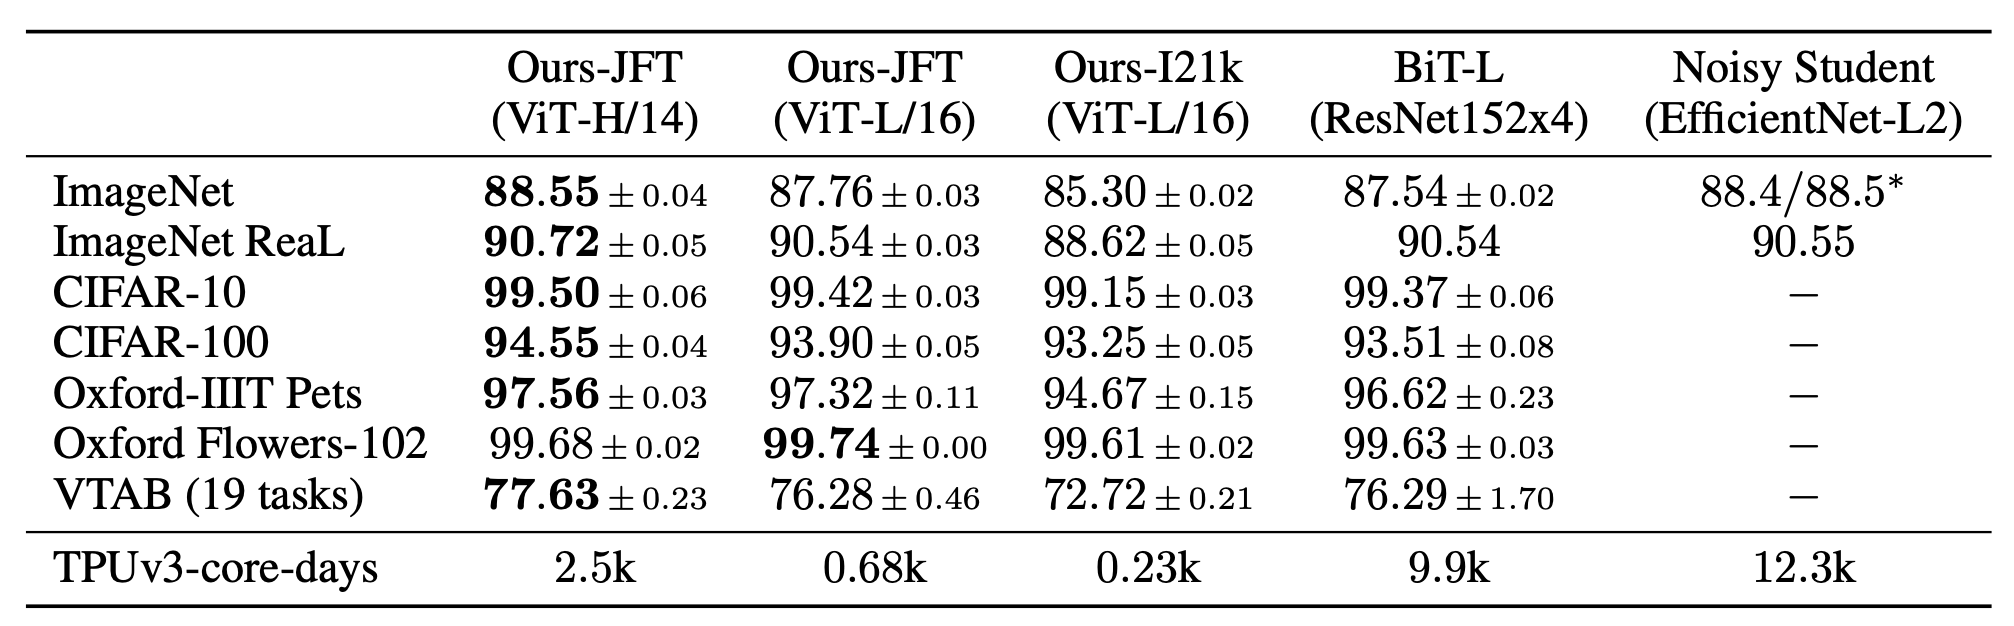
\includegraphics[width=0.8\columnwidth]{picture/The ViT model precision}
		%\captionsetup{font=scriptsize}
		\caption{
			\label{fig: ViT precision} The comparison of the ViT model precision .
		}
	\end{figure}
	
	
	Fig.\ref{fig: ViT precision}中前3列为不同尺度的ViT模型,使用不同的大规模数据集进行预训练,并迁移到各个子任务上的结果。第4列为BiT算法基于JFT-300M数据集预训练后,迁移到各个子任务的结果。第5列为2020年提出的半监督算法 Noisy Student 在 ImageNet 和 ImageNet ReaL 数据集上的结果。
	
	\subsubsection{图像分块嵌入}
	
	在Transformer结构中,输入需要是一个二维的矩阵,矩阵的形状可以表示为$(N,D)$,其中 $N$ 是sequence的长度,而 $D$ 是 sequence 中每个向量的维度。因此,在ViT算法中,首先需要设法将 $H \times W \times C$ 的三维图像转化为 $\left( N,D \right)$ 的二维输入。
	
	ViT中具体实现方式为:将 $H \times W \times C$ 的图像,变为一个 $N \times \left( P^2 * C \right)$ 的序列。这个序列可以看作是一系列展平的图像块,也就是将图像切分成小块后,再将其展平。该序列中一共包含了 $N = \frac{HW}{P^2}$ 个图像块,每个图像块的维度则是 $\left(P^2 * C\right)$。其中 $P$ 是图像块的大小, $C$ 是通道数量。经过如上变换,就可以将 $N$ 视为sequence的长度了。

	但是,此时每个图像块的维度是 $\left(P^2 * C\right)$ ,而我们实际需要的向量维度是 $D$,因此我们还需要对图像块进行 Embedding。Embedding 的方式相对简单,只需要对每个 $\left(P^2 * C\right)$ 的图像块做一个线性变换,将维度压缩为 $D$ 即可。
	
	上述对图像进行分块以及 Embedding 的具体方式如Fig.\ref{fig: Vision Transformer}所示。
	
	\subsection{Data-efficient Image Transformer\cite{touvron2021training}}
	
	ViT 算法要想要获得一个较好的指标,需要先使用 JFT-300 或者 ImageNet-21K 这样的超大规模数据集进行预训练\footnote{JFT-300 和 ImageNet-21K 是两个大规模的图像数据集,一般用于图像分类。
	\begin{itemize}
		\item {}
		JFT-300是一个巨大的图像数据集,包含约 300 亿张图像,是一个真实世界场景的多模态数据集,包含图像和文本数据。
		\item {}
		ImageNet-21K 是 ImageNet 数据集的扩展版本,它包含约 2.1 万个类别(21,841个类别),而传统的 ImageNet 数据集只包含 1000 个类别。
	\end{itemize}
	},然后再迁移到其他中等或较小规模的数据集上。而当不使用像 JFT-300 这样的巨大的数据集时,效果比 CNN 模型差,这反映出 Transformer 结构在 CV 领域的一个局限性。对于大多数的研究者而言,使用如此大规模的数据集意味着需要很昂贵的计算资源,一旦无法获取到这些计算资源,就不能使用这么大规模的数据集进行预训练,就无法复现出算法应有的效果。所以,出于这个动机,作者针对 ViT 算法进行了改进,提出了Data-efficient Image Transformer(DeiT)。
	
	在 DeiT 中,作者在 ViT 的基础上改进了训练策略,并使用了蒸馏学习的方式,只需要在 ImageNet 上进行训练,就可以得到一个有竞争力的 Transformer 模型,而且在单台计算机上,训练时间一般不到3天即可。
	
	如Fig.\ref{fig: DeiT accuracy}所示是DeiT在ImageNet 数据集\footnote{ImageNet 是一个大规模的图像数据集,由斯坦福大学创建。该数据集是计算机视觉中最受欢迎和广泛使用的数据集之一,对于图像分类、目标检测和图像识别等任务都有重要的影响。ImageNet 包含了数百万张高分辨率图像,来自几千个不同的类别。}上与之前 ViT 以及 CNN 算法中的 EfficientNet 的精度对比。其中Fig.\ref{fig: DeiT accuracy}的指标均为在 ImageNet 数据集上进行训练和评估的结果。其中,Ours(Deit) 为使用与 ViT 完全一致的网络结构,但是改进了训练策略;而 Ours⚗(DeiT⚗) 则是在 DeiT 的基础上继续使用了蒸馏学习的方式进行改进。可以看到,ViT 算法在这种中等规模的数据集上,指标\footnote{top-1 accuracy表示模型预测的结果与真实标签匹配的比例,其中“top-1”表示只考虑模型预测的第一个最有可能的类别。}远不如 CNN 网络 EfficientNet,而通过改变训练策略,使用蒸馏学习,网络结构与 ViT 基本一致的 DeiT 性能有了很大的提升,超过了 EfficientNet。
	
	\begin{figure}[htbp]
		% read manual to see what [ht] means and for other possible options
		\centering 
		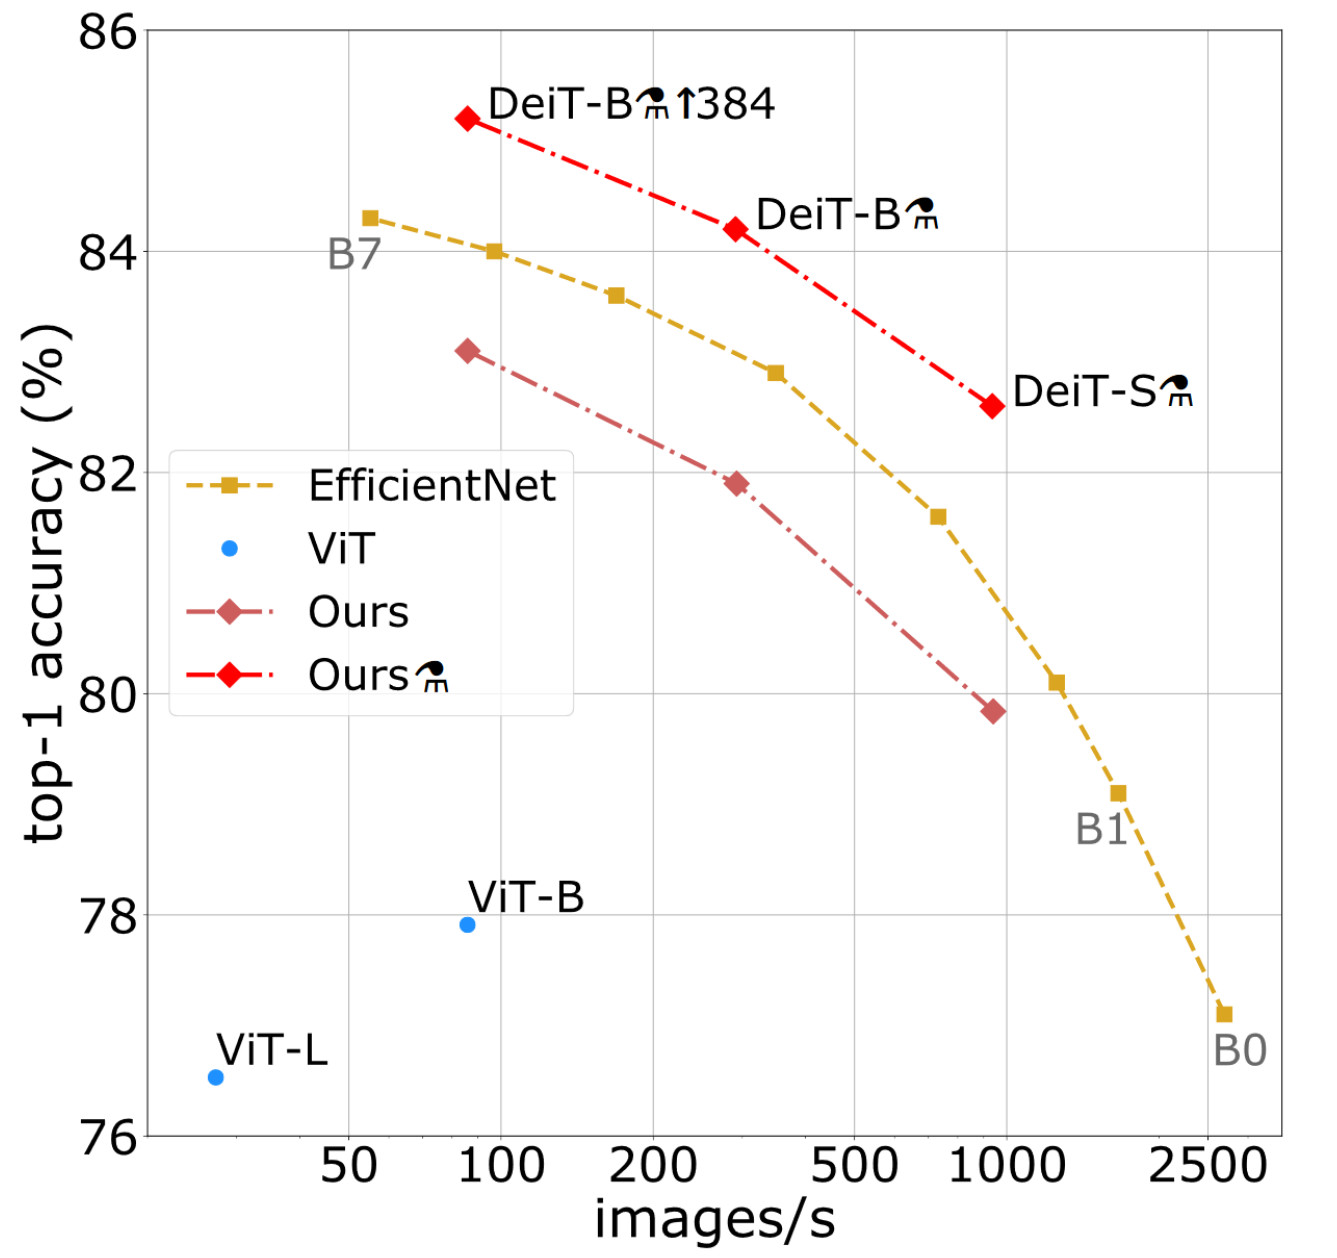
\includegraphics[width=0.5
		\columnwidth]{picture/Accuracy}
		%\captionsetup{font=scriptsize}
		\caption{
			\label{fig: DeiT accuracy} Throughput and accuracy on Imagenet of our method (no external training data). The throughput is measured as the number of images processed per second on a V100 GPU. DeiT-B is identical to ViT-B, but with training adapted to a data-starving regime. It is learned in a few days on one machine. The symbol ⚗ refers to models trained with our transformer-specific distillation. See Table 5 for details and more models.
		}
	\end{figure}
	
	\subsubsection{Network optimization method}
	
	\paragraph{Distilling learning}
	
	蒸馏分为两种,分别是软蒸馏(soft distillation)和硬蒸馏(hard distillation)。软蒸馏就是将学生网络的输出结果与教师网络的 softmax 输出结果取 KL Loss;而硬蒸馏就是将学生网络的输出结果与教师网络的标签取交叉熵损失,公式分别如下所示。在 DeiT 中,分别对网络使用了两种蒸馏策略进行对比实验,最终选择了硬蒸馏方式。
	
	\begin{equation}
		\begin{aligned}
			& L_{global}^{SoftDistill} = \left(1-\lambda\right) \text{L}_{CE}\left(\psi(Z_s), y\right) + \lambda \tau^2 \text{KL}\left(\psi(Z_s/\tau), \psi(Z_t/\tau)\right) \\
			& L_{global}^{HardDistill} = \frac{1}{2} \text{L}_{CE}\left(\psi(Z_s), y\right) + \frac{1}{2} \text{L}_{CE}\left(\psi(Z_s),y_t\right)
		\end{aligned}
		\label{eq: distillation}
	\end{equation}
	
	Eq.\ref{eq: distillation}中,$y_t = argmax_{c} Z_t(c)$.这里的硬标签也可以通过标签平滑技术 (Label smoothing) 转换成软标签,其中真值对应的标签被认为具有 $1-\epsilon$ 的概率,剩余的 $\epsilon$ 则由剩余的类别共享。$\epsilon$ 是一个超参数,这里取0.1。
	
	\paragraph{Network structure}
	
	DeiT 算法相较于 ViT 算法,在网络结构上的优化方式,如Fig.\ref{fig: DeiT-network-structure}所示。
	
	\begin{figure}[htbp]
		% read manual to see what [ht] means and for other possible options
		\centering 
		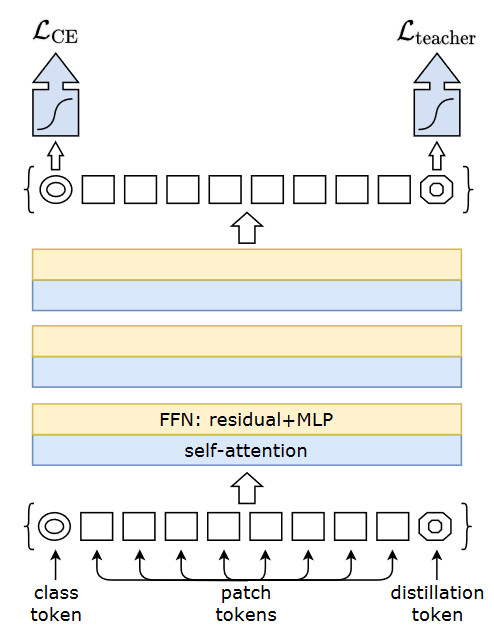
\includegraphics[width=0.5
		\columnwidth]{picture/DeiT-network-structure}
		%\captionsetup{font=scriptsize}
		\caption{
			\label{fig: DeiT-network-structure} Our distillation procedure: we simply include a new distillation token. It interacts with the class and patch tokens through the self-attention layers. This distillation token is employed in a similar fashion as the class token, except that on output of the network its objective is to reproduce the (hard) label predicted by the teacher, instead of true label. Both the class and distillation tokens input to the transformers are learned by back-propagation.
		}
	\end{figure}
	
	通过对比Fig.\ref{fig: DeiT-network-structure}与Fig.\ref{fig: Vision Transformer}中ViT的网络结构可以发现,DeiT 与 ViT 的主要差异在于引入 distillation token,顾名思义,其主要用于网络训练中的蒸馏学习。Distillation token 与 class token 很像,其在 self-attention layers 中会跟 class token 以及图像 patch 不断交互。而 distillation token 与 class token 唯一的区别在于,class token 的目标是跟真实的 label 一致,而 distillation token 是要跟蒸馏学习中教师网络预测的 label 一致。这个 distillation token 允许我们的模型从教师网络的输出中学习,就像在常规的蒸馏中一样,同时也作为一种对 class token 的补充。
	
	由于具有了 distillation token,因此在损失函数方面,DeiT 相较于 ViT 也有了一定的改变:
	
	\begin{itemize}
		\item{}
			在 ViT 算法中,模型的最终输出是使用 class token 进行 softmax 计算,获取预测结果属于各个类别的概率分布。此时,损失函数的计算方式与传统的多分类任务一致,直接使用交叉熵损失即可。
		\item{}
			在 DeiT 算法中,由于使用了蒸馏学习方法,因此在交叉熵损失的基础上,还需要加上一个蒸馏损失。
	\end{itemize}
	
	论文中进行了实验,发现了一个有趣的现象,class token 和 distillation token 是朝着不同的方向收敛的,在开始时,这两个 token 计算余弦相似度只有0.006。随着网络层数的增加,直到最后一层,这两个 token 的余弦相似度变为了0.93。也就可以认为是相似但是不相同的两个 token。
	
	同时,网络为了验证 distillation token 的确给模型添加了某些有益信息,论文中也进行了实验。作者将 distillation token 替换为一个简单的 class token,然后发现,即便这两个 class token 分别进行独立的随机初始化,它们最终也是会随机地收敛到一个几乎一摸一样的结果(余弦相似度为0.999),同时最终性能没有明显提升。网络既会输出 class token 的结果,也会输出 distillation token 的结果,在最终预测时,将两者的 softmax 结果进行相加,即可简单地得到算法的最终预测结果。
	
%%%%%%%%%%%%%%%%%%%%%%%%%%%%%%%%%%%%%%%%%%%%%%%%%%%%%%%%%%%%%%%%%%%%%%%%%%%%%%%%%%%%%%%%%%%%%%%%%%%%
%%%%%%%%%%%%%%%%%%%%%%%%%%%%%%%%%%%%%%%%%%%%%%%%%%%%%%%%%%%%%%%%%%%%%%%%%%%%%%%%%%%%%%%%%%%%%%%%%%%%
%%                                                                                                %% 
%%								          Paper reading                                           %%
%%                                                                                                %%
%%%%%%%%%%%%%%%%%%%%%%%%%%%%%%%%%%%%%%%%%%%%%%%%%%%%%%%%%%%%%%%%%%%%%%%%%%%%%%%%%%%%%%%%%%%%%%%%%%%%
%%%%%%%%%%%%%%%%%%%%%%%%%%%%%%%%%%%%%%%%%%%%%%%%%%%%%%%%%%%%%%%%%%%%%%%%%%%%%%%%%%%%%%%%%%%%%%%%%%%%	

	
	\section{Paper reading}
	
	\subsection{Embedding Fourier for Ultra-High-Definition Low-Light Image Enhancement \cite{li2023embedding}}
	
	本文\footnote{Submitted on 23 Feb 2023}重点研究了图像恢复中最具挑战性的任务之一,即微光图像增强(LLIE),该任务需要联合增强亮度并去除传感器和昏暗环境引起的固有噪声,并通过要求在超高清状态下进行高效处理来提高难度。
	该文提出了UHD LLIE的新解决方案,灵感来自于在傅里叶域中观察到的独特特征。
	
	\subsubsection{Why?}
	
	近年来,随着先进成像传感器和显示器的出现,超高清(UHD)成像技术得到了快速发展。虽然超高清成像提供了广泛的应用,并使图像质量有了显著的不同,但额外的像素也对现有图像处理算法的效率提出了挑战。
	尽管微光图像增强(LLIE)取得了显著进展,但现有方法,在用于处理真实世界的UHD低光图像时显示出明显的缺点。主要有如下四点原因:
	
	\begin{itemize}
		\item {}
			(1) 大多数方法只关注亮度增强,无法去除噪声;
		\item {}
			(2) 一些方法在空间域中同时增强亮度和去噪,导致增强次优;
		\item {}
			(3) 现有方法主要在低分辨率(LR)数据上进行训练,导致与高分辨率(HR)输入不兼容;
		\item {}
			(4) 部分研究采用重结构,因此在处理超高清图像时效率低下。
	\end{itemize}
		
	\subsubsection{Contribution}

	\begin{itemize}
		\item {}
			(1) 提出了一种 UHD LLIE 的新解决方案,灵感来自于在傅里叶域中观察到的独特特征。与现有的LLIE方法相比,所提出的框架在解决超高清环境下亮度增强和噪声去除的联合任务方面表现出了卓越的有效性和效率。
		\item {}
			(2) 我们贡献了第一个超高清 LLIE 数据集,该数据集包含 2150 对 4K 超高清低噪声/正常清晰数据,涵盖了不同的噪声和黑暗级别和场景。
		\item {}
			(3) 对现有的 UHD 数据 LLIE 方法进行了系统分析
	\end{itemize}
	
	\subsubsection{Approach}
	
	\begin{figure}[htbp]
		% read manual to see what [ht] means and for other possible options
		\centering 
		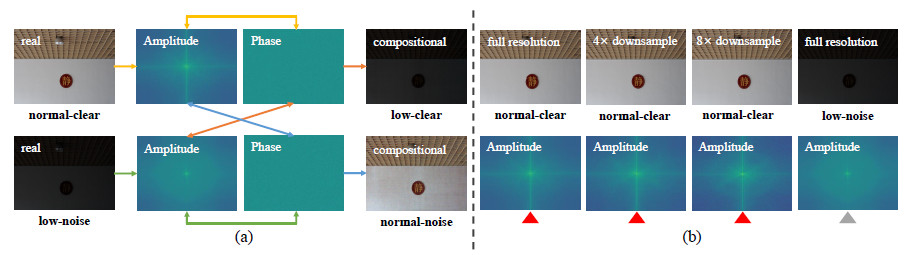
\includegraphics[width=0.8\columnwidth]{picture/Motivations}
		%\captionsetup{font=scriptsize}
		\caption{
			\label{fig: Motivations} Motivations. We observed that (a) luminance and noise can be ‘decomposed’ to a certain extent in the Fourier domain and (b) HR image and its LR versions share similar amplitude patterns. The amplitude and phase are produced by Fast Fourier Transform (FFT) and the compositional images are obtained by Inverse FFT(IFFT). For visualization, we show the amplitude and phase in imagery format with common transformations. Lines of the same color indicate a set of FFT/IFFT transforms. The red triangles mark the similar pattern (obviously different from the gray one). Zoom in for the details and noise. We show more examples and analysis in the Appendix.
		}
	\end{figure}
	
	如Fig.\ref{fig: Motivations}(a)所示,将低光噪声(low-noise)图像的振幅与其对应的正常光清晰(normal-clear)图像的振幅交换,生成正常光噪声(normal-noise)图像和低光清晰(low-clear)图像。结果表明,在傅里叶域中,亮度和噪声都能得到一定程度的分解。特别是,大多数亮度信息表示为振幅和噪声是分阶段显示的。这启发作者在傅里叶域中分别处理亮度和噪声。如Fig.\ref{fig: Motivations}(b)所示,HR正常清晰图像及其LR版本的振幅模式与相应的HR低噪声图像相似而不同。
	
	\subsubsection{Architecture}
		
	\begin{figure}[htbp]
		% read manual to see what [ht] means and for other possible options
		\centering 
		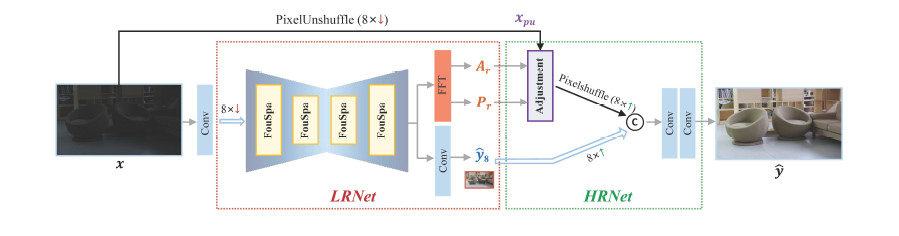
\includegraphics[width=0.8\columnwidth]{picture/UHDFour-architecture}
		%\captionsetup{font=scriptsize}
		\caption{
			\label{fig: UHDFour architecture} \textbf{Overview of UHDFour.} Our approach consists of an LRNet and an HRDNet. The LRNet is an encoder-decoder network that produces 8 $\times$ downsampled result $\hat{y}_{8}$ and the refined amplitude $A_{r}$ and phase $P_{r}$ features. We omit the skip connections for brevity. The HRNet contains an Adjustment Block and the upsampling operation, producing the final result $\hat{y}$. Most computation is conducted in the LRNet.
		}
	\end{figure}
	
	UHDFour 旨在将 UHD 低噪声输入图像 $x \in \mathbb{R}^{H \times W \times C}$ 映射到其对应的正常清除版本 $y \in \mathbb{R}^{H \times W \times C}$,其中$H, W, \text{and} C$分别表示高度、宽度和通道。Fig.\ref{fig: UHDFour architecture}显示了 UHDFour 的架构图, UHDFour 主要由 LRNet 和 HRNet 组成的。
	
	LRNet 的输入首先由 Conv 层嵌入到特征层中。为了降低计算复杂度,通过双线性插值将特征采样到原始分辨率的 1/8 。然后,LR 特征经过一个编码器-解码器网络,该网络包含四个 FouSpa block,带有两个 2 $\times$ downsample和两个2 $\times$ upsample操作,获得输出特征。输出特征分别输入到 FFT 得到细化的振幅 $A_r$ 和相位$P_r$特征,并通过 Conv 层估计 LR 法向清晰图像 $\hat{y}_8 \in \mathbb{R}^{\frac{H}{8} \times \frac{W}{8} \times C}$。
	
	LRNet 的输出与输入相结合,被馈送到 HRNet 。具体来说,首先通过 PixelUnshuffle $\left(8 \times \downarrow\right)$ 将输入 $x$ 重塑为 $x_{pu} \in \mathbb{R}^{H \times W \times C \times 64}$ ,以保留原始信息,然后馈送给一个 Adjustment Block 。通过细化的振幅$A_r$和相位$P_r$特征,调整块产生调整后的特征,这些特征通过Pixelshuffle $\left(8 \times \downarrow\right)$ 重新塑造为输入$x$的原始高度和宽度。最后,通过双线性插值将估计得到的 LR 法线清除图像$\hat{y}_8$调整为原始输入$x$的大小,并与上采样特征相结合,估计出最终的 HR 法线清除图像 $\hat{y}$。
		
	FouSpa Block 和 Adjustment Block 见Fig.\ref{fig: FouSpa and Adjustment}
	
	\begin{figure}[htbp]
		% read manual to see what [ht] means and for other possible options
		\centering 
		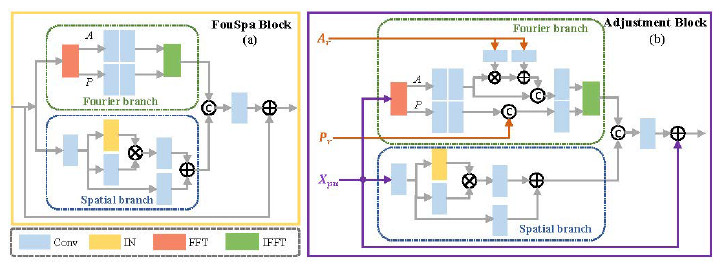
\includegraphics[width=0.8\columnwidth]{picture/FouSpa-and-Adjustment}
		%\captionsetup{font=scriptsize}
		\caption{
			\label{fig: FouSpa and Adjustment} Structures of the FouSpa Block (a) and Adjustment Block (b).
		}
	\end{figure}
	
	已知可知亮度和噪声可以在傅里叶域中分解。因此,作者设计了 FouSpa 块,在傅里叶域并行实现振幅和相位增强,在空间域并行实现特征增强。如Fig.\ref{fig: FouSpa and Adjustment}(a)所示,输入特征分为傅里叶和空间分支。在傅里叶分支中,首先使用FFT来获得振幅分量($A$)和相位分量($P$)。这两个组件分别被$1 \times 1$内核提供给两个 Conv 层。然后,通过 IFFT 将它们转换回空间域,并将它们与半实例归一化 $(HIN)$单元增强的空间特征连接起来。连接的特征被进一步馈送到 Conv 层,然后以残差方式与输入特征结合。
	
	Adjustment Block 是HRNet的主要结构,具有轻量化的特点。如Fig.\ref{fig: FouSpa and Adjustment}(b)所示,Adjustment Block 与 FouSpa Block 具有类似的结构。不同的是,在傅里叶分支中,利用从 LRNet 获得的细化的振幅 $A_r$ 特征,使用空间特征变换(SFT)通过简单的仿射变换来调制输入 $x_{pu}$ 的振幅特征。注意,由于相位的周期性,无法对其进行调制。
	
	\subsubsection{UHD-LL Dataset}
	
	作者收集了一个真正的低噪声/正常清除成对图像数据集,其中包含 2150 对以8bit sRGB格式保存的 4K UHD 数据。图5中显示了几个示例。

	\begin{figure}[htbp]
		% read manual to see what [ht] means and for other possible options
		\centering 
		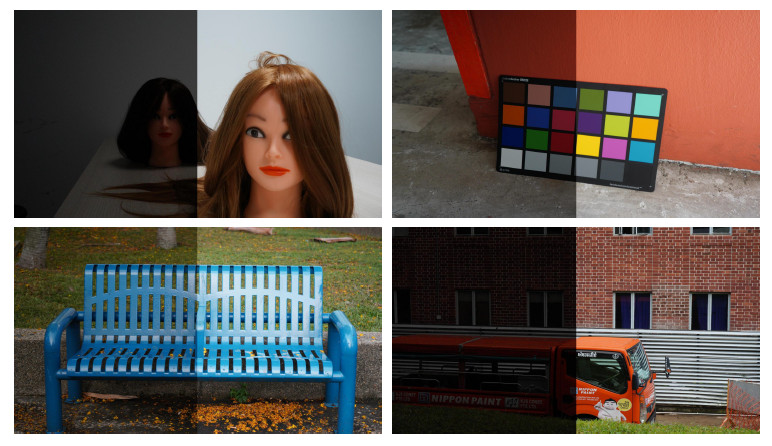
\includegraphics[width=0.5\columnwidth]{picture/Dataset}
		%\captionsetup{font=scriptsize}
		\caption{
			\label{fig: UHD-LL} Samples from the proposed UHD-LL
			dataset.
		}
	\end{figure}
	
	作者将 UHD-LL 数据集分为两部分:2000对用于训练,115对用于测试。训练和测试分区在它们的场景和数据中是独占的。作者还确保了训练和测试分割之间像素强度分布的一致性。UHD-LL 数据集与现有的配对微光图像数据集之间的比较如Tab.\ref{tab: Datasets comparison}所示。LOL数据集(两个版本:LOL-v1: 500张图片;LOL-v2: 789张图像)与UHD-LL数据集最相关,因为两者都专注于带有噪声的真实微光图像。LOL-v2包含LOL-v1的所有图像。与LOL数据集相比,UHD-LL数据集具有更广泛的集合,其中考虑了来自丰富类型场景的不同黑暗和噪音水平。
	
	\begin{table}[!htbp]
		\centering
		\small
		\caption{\label{tab: Datasets comparison}
			Comparison between classic LLIE datasets
			and our UHD-LL dataset. ‘Number’: the number of
			paired images. ‘Resolution’: the average resolution of the
			dataset. ‘Noise’: low-light images contain noise. ‘Real’:
			both low-light images and GT are acquired in real scenes.} %表格的标题
		%\resizebox{\textwidth}{!}{ %按照宽度调整调整表格大小
			\begin{tabular}{>{\centering\arraybackslash}m{2.6cm}|c|c|c|c}
				
				\hline
				
				\textbf{Dataset} & \textbf{Number} & \textbf{Resolution} & \textbf{Noise} & \textbf{Real} \\
				
				\hline
				
				SID(RAW) & 5094 & \makecell{4240 $\times$ 2832 \\ 6000 $\times$ 4000} & \checkmark & \checkmark \\ 
				MIT-Adobe FiveK & 5000 & 4000 $\times$ 2500 &  &  \\ 
				Exposure-Errors  & 24000 & 1000 $\times$ 900 &  &  \\
				LOL & 500/789 & 600 $\times$ 400 & \checkmark & \checkmark \\
				\textbf{UHD-LL(Ours)} & \textbf{2150} & \textbf{3840 $\times$ 2160} & \checkmark & \checkmark \\
				
				\hline
				
			\end{tabular}
			%}
		\captionsetup{font=scriptsize} %设置标题字体与表格字体一致
	\end{table}
	
	\section{个人工作进展}
	
	\subsection{思考}
	
	\begin{itemize}
		\item [(1)] 目前很大一部分工作还是把 Transformer 和现有的 CNN 工作结合在一起,如 ViT 其实也是有 Hybrid Architecture (将由 ResNet 提取的特征图馈入 ViT 而非原始图像)。而对于检测和分割这类问题,CNN 方法相对已经非常成熟,难以用 Transformer 一下子完全替换掉。目前绝大部分的工作大都是 CNN 和 Transformer 的混合体,这其中有速度和效果的双重考虑。另外,也要考虑到 如果输入较大分辨率的图像,Transformer 的计算量会很大,所以 ViT 的输入并不是 Pixel,而是小 Patch。
		
		\item [(2)] 目前的工作已经证明:一个三层神经网络可以逼近任何一个非线性函数,前提是参数足够大,而且更重要的是找到一个好的训练方法。
		
	\end{itemize}

	
	\section{下周工作计划}
	
	(1) 使用百度的paddlepaddle库复现ViT和DeiT。
	
	(2) 了解Swin Transformer。
	%	\section{Analysis}
	
	%	In this section you will need to show your experimental results. Use tables and
	%	graphs when it is possible. Table~\ref{tbl:bins} is an example.
	
	%	\begin{table}[ht]
		%		\begin{center}
			%			\caption{Every table needs a caption.}
			%			\label{tbl:bins} % spaces are big no-no withing labels
			%			\begin{tabular}{|ccc|} 
				%				\hline
				%				\multicolumn{1}{|c}{$x$ (m)} & \multicolumn{1}{c|}{$V$ (V)} & \multicolumn{1}{c|}{$V$ (V)} \\
				%				\hline
				%				0.0044151 &   0.0030871 &   0.0030871\\
				%				0.0021633 &   0.0021343 &   0.0030871\\
				%				0.0003600 &   0.0018642 &   0.0030871\\
				%				0.0023831 &   0.0013287 &   0.0030871\\
				%				\hline
				%			\end{tabular}
			%		\end{center}
		%	\end{table}
	%	
	%	Analysis of equation~\ref{eq:aperp} shows ...
	%	
	%	Note: this section can be integrated with the previous one as long as you
	%	address the issue. Here explain how you determine uncertainties for different
	%	measured values. Suppose that in the experiment you make a series of
	%	measurements of a resistance of the wire $R$ for different applied voltages
	%	$V$, then you calculate the temperature from the resistance using a known
	%	equation and make a plot  temperature vs. voltage squared. Again suppose that
	%	this dependence is expected to be linear~\cite{Cyr}, and the proportionality coefficient
	%	is extracted from the graph. Then what you need to explain is that for the
	%	resistance and the voltage the uncertainties are instrumental (since each
	%	measurements in done only once), and they are $\dots$. Then give an equation
	%	for calculating the uncertainty of the temperature from the resistance
	%	uncertainty. Finally explain how the uncertainty of the slop of the graph was
	%	found (computer fitting, graphical method, \emph{etc}.)
	%	
	%	If in the process of data analysis you found any noticeable systematic
	%	error(s), you have to explain them in this section of the report.
	%	
	%	It is also recommended to plot the data graphically to efficiently illustrate
	%	any points of discussion. For example, it is easy to conclude that the
	%	experiment and theory match each other rather well if you look at
	%	Fig.~\ref{fig:samplesetup} and Fig.~\ref{fig:exp_plots}.
	%	
	%	\begin{figure}[ht] 
		%		\centering
		%		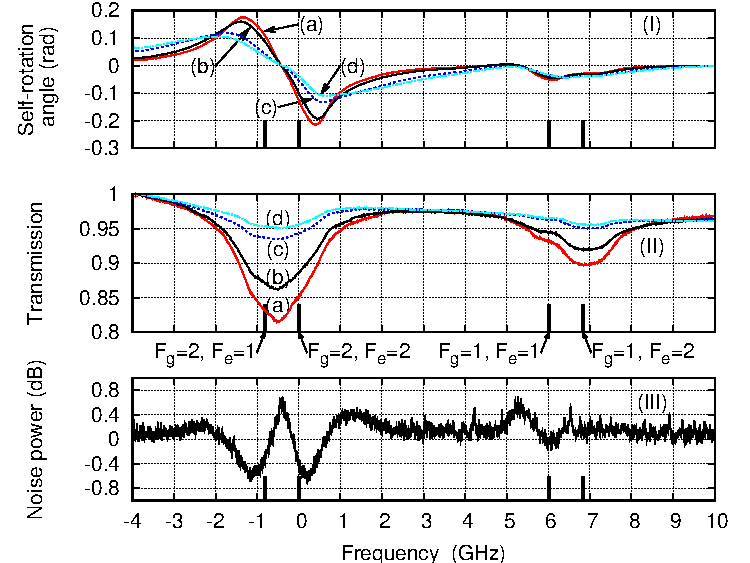
\includegraphics[width=0.5\columnwidth]{sr_squeezing_vs_detuning}
		%		
		%		% some figures do not need to be too wide
		%		\caption{
			%			\label{fig:exp_plots}  
			%			Every plot must have axes labeled.
			%		}
		%	\end{figure}
	
	
	%	\section{Conclusions}
	%	Here you briefly summarize your findings.
	
	%++++++++++++++++++++++++++++++++++++++++
	% References section will be created automatically 
	% with inclusion of "thebibliography" environment
	% as it shown below. See text starting with line
	% \begin{thebibliography}{99}
		% Note: with this approach it is YOUR responsibility to put them in order
		% of appearance.
		
		\renewcommand{\refname}{References}
		
		
		%	\begin{thebibliography}{00}
			
			%		\bibitem{b1}\label{cite:b1}
			%		W. Wang, C. Wei, W. Yang and J. Liu, "GLADNet: Low-Light Enhancement Network with Global Awareness," 2018 13th IEEE International Conference on Automatic Face \& Gesture Recognition (FG 2018), Xi'an, China, 2018, pp. 751-755, DOI: 10.1109/FG.2018.00118.
			
			%		\bibitem{b2}\label{cite:b2}
			%		A.\ Mahajan, K.\ Somaraj and M. Sameer, "Adopting Artificial Intelligence Powered ConvNet To Detect Epileptic Seizures," 2020 IEEE-EMBS Conference on Biomedical Engineering and Sciences (IECBES), Langkawi Island, Malaysia, 2021, pp. 427-432, DOI: 10.1109/IECBES48179.2021.9398832.
			
			%		\bibitem{Cyr}
			%		N.\ Cyr, M.\ T$\hat{e}$tu, and M.\ Breton,
			% "All-optical microwave frequency standard: a proposal,"
			%		IEEE Trans.\ Instrum.\ Meas.\ \textbf{42}, 640 (1993).
			
			
			
			%	\end{thebibliography}
		
		\bibliographystyle{unsrt}
		\bibliography{reference}
		
		
	\end{document}
